\tikzstyle{cell} = [ font={\huge\bfseries}, shape=circle,  text=black, draw=black!55, align=center]
\tikzstyle{pvalue} = [draw, fill=blue!50,outer sep=7,inner sep=7,line width=1]
\tikzstyle{ovalue} = [draw, fill=red!50,outer sep=7,inner sep=7,line width=1]
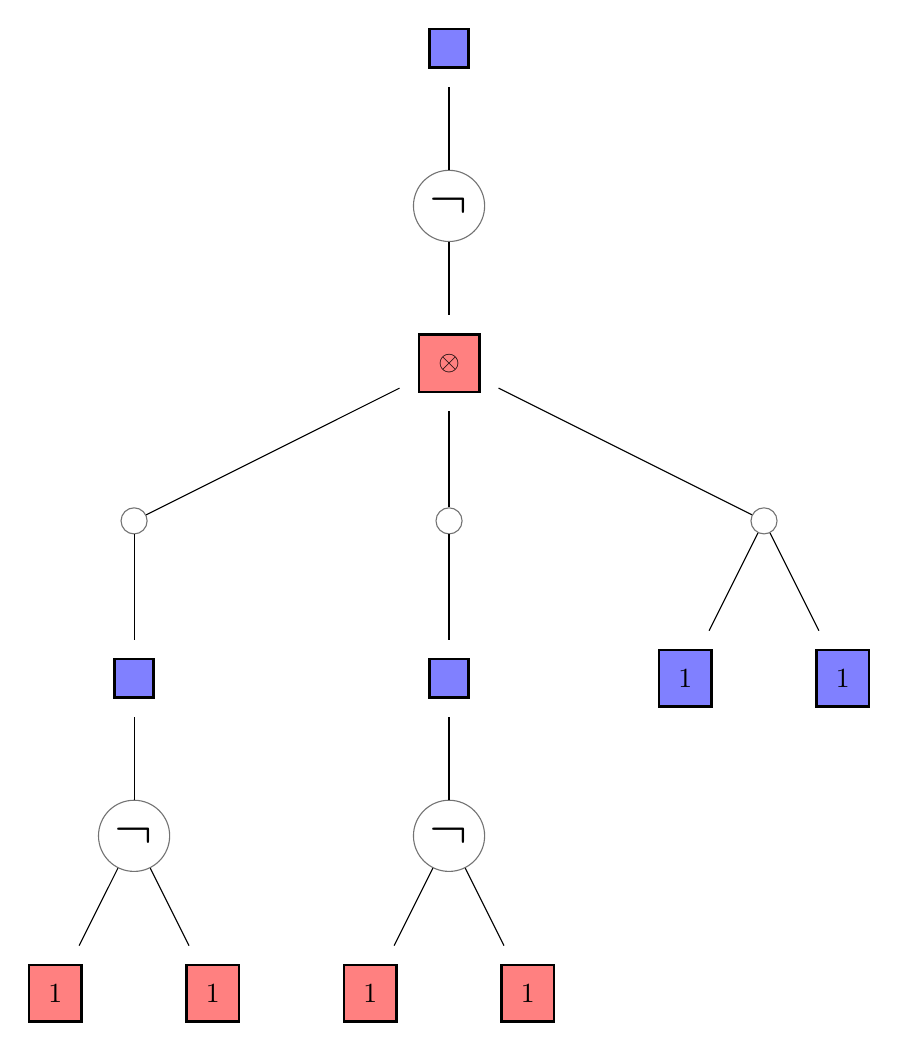
\begin{tikzpicture}

\node [cell] (v2) at (0,5) {$\neg$};
\node [ovalue] (v3) at (0,3) {$\otimes$};
\node [pvalue] (v1) at (0,7) {};
\node [cell] (v4) at (-4,1) {};
\node [cell] (v5) at (0,1) {};
\node [cell] (v6) at (4,1) {};
\node [pvalue] (v7) at (-4,-1) {};
\node [pvalue] (v11) at (0,-1) {};
\node [pvalue] (v15) at (3,-1) {$1$};
\node [pvalue] (v16) at (5,-1) {$1$};
\node [cell] (v8) at (-4,-3) {$\neg$};
\node [cell] (v12) at (0,-3) {$\neg$};
\node [ovalue] (v9) at (-5,-5) {$1$};
\node [ovalue] (v10) at (-3,-5) {$1$};
\node [ovalue] (v13) at (-1,-5) {$1$};
\node [ovalue] (v14) at (1,-5) {$1$};
\draw  (v1) edge (v2);
\draw  (v2) edge (v3);
\draw  (v3) edge (v4);
\draw  (v3) edge (v5);
\draw  (v3) edge (v6);
\draw  (v4) edge (v7);
\draw  (v7) edge (v8);
\draw  (v8) edge (v9);
\draw  (v8) edge (v10);
\draw  (v5) edge (v11);
\draw  (v11) edge (v12);
\draw  (v12) edge (v13);
\draw  (v12) edge (v14);
\draw  (v6) edge (v15);
\draw  (v6) edge (v16);
\end{tikzpicture}